% this is a simplified version of
% https://github.com/yihui/knitr/blob/master/inst/examples/knitr-beamer.Rnw
%
% Update 2015-07-22
% This is no longer simple. The above statement is a lie.
% \documentclass[handout]{beamer}
\documentclass{beamer}\usepackage[]{graphicx}\usepackage[]{color}
%% maxwidth is the original width if it is less than linewidth
%% otherwise use linewidth (to make sure the graphics do not exceed the margin)
\makeatletter
\def\maxwidth{ %
  \ifdim\Gin@nat@width>\linewidth
    \linewidth
  \else
    \Gin@nat@width
  \fi
}
\makeatother

\definecolor{fgcolor}{rgb}{0.345, 0.345, 0.345}
\newcommand{\hlnum}[1]{\textcolor[rgb]{0.686,0.059,0.569}{#1}}%
\newcommand{\hlstr}[1]{\textcolor[rgb]{0.192,0.494,0.8}{#1}}%
\newcommand{\hlcom}[1]{\textcolor[rgb]{0.678,0.584,0.686}{\textit{#1}}}%
\newcommand{\hlopt}[1]{\textcolor[rgb]{0,0,0}{#1}}%
\newcommand{\hlstd}[1]{\textcolor[rgb]{0.345,0.345,0.345}{#1}}%
\newcommand{\hlkwa}[1]{\textcolor[rgb]{0.161,0.373,0.58}{\textbf{#1}}}%
\newcommand{\hlkwb}[1]{\textcolor[rgb]{0.69,0.353,0.396}{#1}}%
\newcommand{\hlkwc}[1]{\textcolor[rgb]{0.333,0.667,0.333}{#1}}%
\newcommand{\hlkwd}[1]{\textcolor[rgb]{0.737,0.353,0.396}{\textbf{#1}}}%

\usepackage{framed}
\makeatletter
\newenvironment{kframe}{%
 \def\at@end@of@kframe{}%
 \ifinner\ifhmode%
  \def\at@end@of@kframe{\end{minipage}}%
  \begin{minipage}{\columnwidth}%
 \fi\fi%
 \def\FrameCommand##1{\hskip\@totalleftmargin \hskip-\fboxsep
 \colorbox{shadecolor}{##1}\hskip-\fboxsep
     % There is no \\@totalrightmargin, so:
     \hskip-\linewidth \hskip-\@totalleftmargin \hskip\columnwidth}%
 \MakeFramed {\advance\hsize-\width
   \@totalleftmargin\z@ \linewidth\hsize
   \@setminipage}}%
 {\par\unskip\endMakeFramed%
 \at@end@of@kframe}
\makeatother

\definecolor{shadecolor}{rgb}{.97, .97, .97}
\definecolor{messagecolor}{rgb}{0, 0, 0}
\definecolor{warningcolor}{rgb}{1, 0, 1}
\definecolor{errorcolor}{rgb}{1, 0, 0}
\newenvironment{knitrout}{}{} % an empty environment to be redefined in TeX

\usepackage{alltt}
\mode<presentation>
{
  \usetheme{default}      % or try Darmstadt, Madrid, Warsaw, ...
  \usecolortheme{dove}    % or try albatross, beaver, crane, ...
  \usefonttheme{default}  % or try serif, structurebold, ...

  % Setting the empty braces turns off the navigation symbols
  \setbeamertemplate{navigation symbols}{}

  % I believe these two lines make it so the slides are counted at the bottom.
  \setbeamertemplate{caption}[numbered]
  \setbeamertemplate{footline}[frame number]

  % These have no purpose or place in this presentation.
  \definecolor{links}{HTML}{2A1B81}
  \hypersetup{colorlinks,linkcolor=,urlcolor=links}
}

% Used for bibliography at the end.
\usepackage{subfig}
\usepackage{appendixnumberbeamer}
\usepackage[backend=bibtex, style=authoryear-comp]{biblatex}
\addbibresource{citations.bib}

% Shaded text box color. This defines beige or tan
% http://www.slideshare.net/linjaaho/how-to-make-boxed-text-with-latex
\usepackage{framed, color}
\definecolor{shadecolor}{HTML}{d2b48c}

% This is the color for the "QUESTIONS" header
\definecolor{mygreen}{HTML}{558046}

\usepackage[absolute,overlay]{textpos}

% Package for overlaying images and drawing arrows, circles, etc.
% http://tex.stackexchange.com/a/34928/77699
\usepackage{tikz}

% This bit gives attribution to photos.
% http://tex.stackexchange.com/a/48485/77699
\setbeamercolor{framesource}{fg=white}
\setbeamerfont{framesource}{size=\footnotesize}
\newcommand{\source}[2]{\begin{textblock*}{4cm}(8.7cm,8.6cm)
    \begin{beamercolorbox}[ht=0.5cm,right]{framesource}
        \usebeamerfont{framesource}\usebeamercolor[#2]{framesource}{#1}
    \end{beamercolorbox}
\end{textblock*}}

% A whole bunch of stuff for citations so that they would end up in a
% bibliography.
\newcommand{\mycitep}[1]{\scriptsize{\textcolor{gray}{(\citeauthor{#1}, \citeyear{#1})}}}
\newcommand{\mycite}[1]{\scriptsize{\textcolor{gray}{\citeauthor{#1}, \citeyear{#1}}}}
\newcommand{\foocite}[1]{\footnote{\scriptsize{\textcolor{gray}{\citeauthor{#1}, \citeyear{#1}}}}}
% I really have no clue why this line is here.
\newcommand{\btVFill}{\vskip0pt plus 1filll}
\renewcommand*{\bibfont}{\footnotesize}

% Setup Chunks




\IfFileExists{upquote.sty}{\usepackage{upquote}}{}
\begin{document}

\title{Evidence for at least two introductions\\ of the sudden oak death pathogen\\ into Oregon forests}

\author{\textbf{ZN Kamvar}, MM Larsen, AM Kanaskie, \\
EM Hansen, and NJ Gr{\"u}nwald}

\date{APS Annual Meeting, Pasadena, CA\\August 02, 2015}
\maketitle

%''''''''''''''''''''''''''''''''''''''''''''''''''''''''''''''''''''''''''''''\
%------------------------------------------------------------------------------|
% \begin{frame}
% 	\frametitle{Outline}
% 	\centering
% 	\LARGE
% 	\tableofcontents
% \end{frame}
%------------------------------------------------------------------------------|
%,,,,,,,,,,,,,,,,,,,,,,,,,,,,,,,,,,,,,,,,,,,,,,,,,,,,,,,,,,,,,,,,,,,,,,,,,,,,,,/

% Removing the blank line as a header.
% http://tex.stackexchange.com/a/33288/77699
\setbeamertemplate{headline}{}

% Setting a custom background image
% http://tex.stackexchange.com/a/78470/77699
\setbeamertemplate{background}
{\includegraphics[width=\paperwidth,height=\paperheight]{../OR_epidemic.png}}
\source{Mike McWilliams, ODF}{white}


\section{What is Sudden Oak Death?}
%''''''''''''''''''''''''''''''''''''''''''''''''''''''''''''''''''''''''''''''\
%------------------------------------------------------------------------------|
\begin{frame}
	\begin{center}
		\begin{shaded}
		 	\Large{\bf \sc Background}\\
		 	\Large{\bf What is Sudden Oak Death?}
	 	\end{shaded}
	\end{center}
\end{frame}
%------------------------------------------------------------------------------|
%,,,,,,,,,,,,,,,,,,,,,,,,,,,,,,,,,,,,,,,,,,,,,,,,,,,,,,,,,,,,,,,,,,,,,,,,,,,,,,/

% Resetting the default background and header
\setbeamertemplate{background}[default]
\setbeamertemplate{headline}[default]

% Setting the caption to be tiny again
\setbeamerfont{framesource}{size=\tiny}


%''''''''''''''''''''''''''''''''''''''''''''''''''''''''''''''''''''''''''''''\
%------------------------------------------------------------------------------|
\begin{frame}
\frametitle{\em Phytophthora ramorum}
\begin{columns}[T]
	\begin{column}{0.4\textwidth}
		\begin{itemize}
			\large
			\item Non-native
			\item $>100$ hosts
			\item Introduced into\\ CA Bay Area\\ circa mid 1990’s
			\item 4 Clonal lineages
			\begin{itemize}
				\item \textbf{NA1}, NA2
				\item EU1, EU2
			\end{itemize}
			\item \textbf{Spread to Oregon\\ before 2001} \\ \mycitep{hansen2008epidemiology}
		\end{itemize}
	\end{column}
	\begin{column}{0.6\textwidth}
		\centering
		\includegraphics[height=0.75\paperheight,keepaspectratio]{../SuddenOakDeath05_Jennifer_Parke.jpg}
		\source{Photo: Jennifer Parke, OSU}{gray}
	\end{column}
\end{columns}
\end{frame}
%------------------------------------------------------------------------------|
%,,,,,,,,,,,,,,,,,,,,,,,,,,,,,,,,,,,,,,,,,,,,,,,,,,,,,,,,,,,,,,,,,,,,,,,,,,,,,,/

% Setting attribution size larger for background slide
\setbeamerfont{framesource}{size=\footnotesize}
\setbeamertemplate{background}
{\includegraphics[width=\paperwidth,height=\paperheight]{../OR_epidemic.png}}
\source{Mike McWilliams, ODF}{white}

\section{Curry County Epidemic 2001 -- Present}
%''''''''''''''''''''''''''''''''''''''''''''''''''''''''''''''''''''''''''''''\
%------------------------------------------------------------------------------|
\begin{frame}[t]
	\begin{center}
		\begin{shaded}
	  		\Large{\bf Curry County Epidemic\\2001 -- Present}
	  	\end{shaded}
 	\end{center}
\end{frame}
%------------------------------------------------------------------------------|
%,,,,,,,,,,,,,,,,,,,,,,,,,,,,,,,,,,,,,,,,,,,,,,,,,,,,,,,,,,,,,,,,,,,,,,,,,,,,,,/

\setbeamertemplate{background}[default]
\setbeamertemplate{headline}[default]


%''''''''''''''''''''''''''''''''''''''''''''''''''''''''''''''''''''''''''''''\
%------------------------------------------------------------------------------|
\begin{frame}[allowpagebreak,T]

% fig.show = "hide" is important here because knitr does not handle rescaling
% plots very well. It will squish them. Setting keepaspectratio prevents
% squishing.

	\centering
	\includegraphics[keepaspectratio, height=\paperheight]{figure/insetplot-1.pdf}
	\vfill
\end{frame}
%------------------------------------------------------------------------------|
%,,,,,,,,,,,,,,,,,,,,,,,,,,,,,,,,,,,,,,,,,,,,,,,,,,,,,,,,,,,,,,,,,,,,,,,,,,,,,,/


%''''''''''''''''''''''''''''''''''''''''''''''''''''''''''''''''''''''''''''''\
%------------------------------------------------------------------------------|
\begin{frame}



% Overlayed picture
% http://tex.stackexchange.com/a/34928/77699
\centering
\begin{tikzpicture}
  \node (img1) at (0, 0){
  \includegraphics[keepaspectratio, height=0.95\paperheight]{figure/brookings-1.pdf}};
  \node (img2) at (3, 3) {\includegraphics[height=3cm]{../kanaskie.jpg}};
\end{tikzpicture}

\end{frame}
%------------------------------------------------------------------------------|
%,,,,,,,,,,,,,,,,,,,,,,,,,,,,,,,,,,,,,,,,,,,,,,,,,,,,,,,,,,,,,,,,,,,,,,,,,,,,,,/


% These chunks lie outside of the frame because they can.




\setbeamertemplate{headline}{}


%''''''''''''''''''''''''''''''''''''''''''''''''''''''''''''''''''''''''''''''\
%------------------------------------------------------------------------------|
\begin{frame}[allowpagebreak,T]

	\begin{columns}[allowpagebreak,T]
		\begin{column}{0.5\paperwidth}
			\centering
			\includegraphics[keepaspectratio,width=0.48\paperwidth]{figure/2001-1.pdf}
		\end{column}
		\begin{column}{0.5\paperwidth}
			\centering
			\includegraphics[keepaspectratio,width=0.48\paperwidth]{figure/2005-1.pdf}
		\end{column}
	\end{columns}

\end{frame}
%------------------------------------------------------------------------------|
%,,,,,,,,,,,,,,,,,,,,,,,,,,,,,,,,,,,,,,,,,,,,,,,,,,,,,,,,,,,,,,,,,,,,,,,,,,,,,,/






%''''''''''''''''''''''''''''''''''''''''''''''''''''''''''''''''''''''''''''''\
%------------------------------------------------------------------------------|
\begin{frame}[allowpagebreak,T]

	\begin{columns}[allowpagebreak,T]
		\begin{column}{0.5\paperwidth}
			\centering
			\includegraphics[keepaspectratio,width=0.48\paperwidth]{figure/2011-1.pdf}
		\end{column}
		\begin{column}{0.5\paperwidth}
			\centering
			\only<2>{
				\includegraphics[keepaspectratio,width=0.48\paperwidth]{figure/2014-1.pdf}
			}
		\end{column}
	\end{columns}

\end{frame}
%------------------------------------------------------------------------------|
%,,,,,,,,,,,,,,,,,,,,,,,,,,,,,,,,,,,,,,,,,,,,,,,,,,,,,,,,,,,,,,,,,,,,,,,,,,,,,,/


\setbeamerfont{framesource}{size=\tiny}

\section{Research Questions}
%''''''''''''''''''''''''''''''''''''''''''''''''''''''''''''''''''''''''''''''\
%------------------------------------------------------------------------------|
\begin{frame}[allowpagebreak,T]
\begin{columns}[allowpagebreak,T]
	\begin{column}{0.5\textwidth}
		\begin{center}
			\Large{\bf Curry County epidemic}
		\end{center}
		\begin{itemize}
			\item 2001 -- present
			\item Aerial survey detection
			\item \textbf{Aggressive Management} {\mycitep{hansen2008epidemiology}}
			\item \textbf{NA1} clonal lineage
		\end{itemize}
		\begin{center}
			\color{mygreen}
			\only<2->{\Large{\bf Questions}}
		\end{center}
		\begin{enumerate}[<+->]
			\uncover<3->{\item New lineages introduced?}
			\uncover<4->{\item Multiple introductions?}
			\uncover<5->{\item Nursery = source?}
		\end{enumerate}
	\end{column}
	\begin{column}{0.5\textwidth}\centering
		\includegraphics[height=0.75\paperheight,keepaspectratio]{../groundcrew.png}
		\source{Photo: ODF}{gray}
	\end{column}
\end{columns}
\end{frame}
%------------------------------------------------------------------------------|
%,,,,,,,,,,,,,,,,,,,,,,,,,,,,,,,,,,,,,,,,,,,,,,,,,,,,,,,,,,,,,,,,,,,,,,,,,,,,,,/


\setbeamerfont{framesource}{size=\footnotesize}
\setbeamertemplate{background}
{\includegraphics[width=\paperwidth,height=\paperheight]{../OR_epidemic.png}}
\source{Mike McWilliams, ODF}{white}

\section{Methods and Results}
%''''''''''''''''''''''''''''''''''''''''''''''''''''''''''''''''''''''''''''''\
%------------------------------------------------------------------------------|
\begin{frame}
	\begin{center}
	\begin{shaded}
  \Large{\bf \sc Methods and Results}
  \end{shaded}

  \end{center}
\end{frame}
%------------------------------------------------------------------------------|
%,,,,,,,,,,,,,,,,,,,,,,,,,,,,,,,,,,,,,,,,,,,,,,,,,,,,,,,,,,,,,,,,,,,,,,,,,,,,,,/

\setbeamertemplate{background}[default]


\subsection*{Methods}
%''''''''''''''''''''''''''''''''''''''''''''''''''''''''''''''''''''''''''''''\
%------------------------------------------------------------------------------|
\begin{frame}[allowpagebreak,T]

	\begin{columns}[allowpagebreak,c]
		\begin{column}{0.5\paperwidth}
			\centering
	        \begin{tikzpicture}
	        	% This is a complicated little maneuver. Here, I'm showing an
	        	% image and then drawing a red arrow pointing to a specific
	        	% point. The coordinates in the parens represent the y and the x
	        	% positions, respectively. The first set represents the arrow
	        	% head and the second represents the tail The fact that there is
	        	% a little picture of an arrow indicates that it will be so.
	        	%
	        	% http://cremeronline.com/LaTeX/minimaltikz.pdf
	            \node at (0,0) {\includegraphics[keepaspectratio,width=0.48\paperwidth]{figure/dataplot-1.pdf}};
	            \draw<6>[<-, red, line width=12] (-2.1, 2.35) -- (0, 2.35);
        	\end{tikzpicture}

		\end{column}
		\begin{column}{0.5\paperwidth}
			\centering
			\LARGE{\bf Data\\}
			\begin{itemize}
				\item<2-> 512 forest samples
				\begin{itemize}
					\bf
					\item<2-> 70 MLG
				\end{itemize}
				\item<3-> 5 SSR loci
				\item<4-> 216 nursery samples \mycitep{goss2009population}
				\begin{itemize}
					\bf
					\item<4-> 40 MLG
					\item<4-> 12 shared w/ forest
				\end{itemize}
				\item<5-> Missing years (2005--2010) \only<5->{\foocite{peterson2015temporal}}
				\item<6-> 2011 Anomaly
			\end{itemize}
		\end{column}
	\end{columns}

\end{frame}
%------------------------------------------------------------------------------|
%,,,,,,,,,,,,,,,,,,,,,,,,,,,,,,,,,,,,,,,,,,,,,,,,,,,,,,,,,,,,,,,,,,,,,,,,,,,,,,/



%''''''''''''''''''''''''''''''''''''''''''''''''''''''''''''''''''''''''''''''\
%------------------------------------------------------------------------------|
\begin{frame}[allowpagebreak,T]
	\frametitle{Methods}
	\begin{itemize}
		\Large
		\item<1-> \textbf{New Lineage Detection}
		\begin{itemize}
			\Large
			\item<1-> 14 diagnostic microsatellites
		\end{itemize}
		\item<2-> \textbf{Multiple Introductions \& Nursery Contribution}
		\begin{itemize}
			\Large
			\item<3-> Discriminant Analysis of Principal Components (DAPC)\\ \mycitep{jombart2010discriminant}
			\item<4-> Bootstrap Analysis
			\begin{itemize}
				\large
				\item<4-> Nei's distance \mycitep{nei1973analysis}
			\end{itemize}
			\item<5-> Minimum Spanning Networks (MSNs)
			\begin{itemize}
				\large
				\item<5-> Bruvo's distance \mycitep{bruvo2004simple}
			\end{itemize}
		\end{itemize}
	\end{itemize}
\end{frame}
%------------------------------------------------------------------------------|
%,,,,,,,,,,,,,,,,,,,,,,,,,,,,,,,,,,,,,,,,,,,,,,,,,,,,,,,,,,,,,,,,,,,,,,,,,,,,,,/


\subsection*{Results}
%''''''''''''''''''''''''''''''''''''''''''''''''''''''''''''''''''''''''''''''\
%------------------------------------------------------------------------------|
\begin{frame}[allowpagebreak,T]
	\frametitle{DAPC of forest populations}
	\centering
	\includegraphics[keepaspectratio, width=0.85\paperwidth]{../DAPC.png}
\end{frame}
%------------------------------------------------------------------------------|
%,,,,,,,,,,,,,,,,,,,,,,,,,,,,,,,,,,,,,,,,,,,,,,,,,,,,,,,,,,,,,,,,,,,,,,,,,,,,,,/


%''''''''''''''''''''''''''''''''''''''''''''''''''''''''''''''''''''''''''''''\
%------------------------------------------------------------------------------|
\begin{frame}[allowpagebreak,T]
	\frametitle{MSN of forest populations}
	\centering
    \begin{tikzpicture}
	    \node[anchor=north east] at (0, 0) {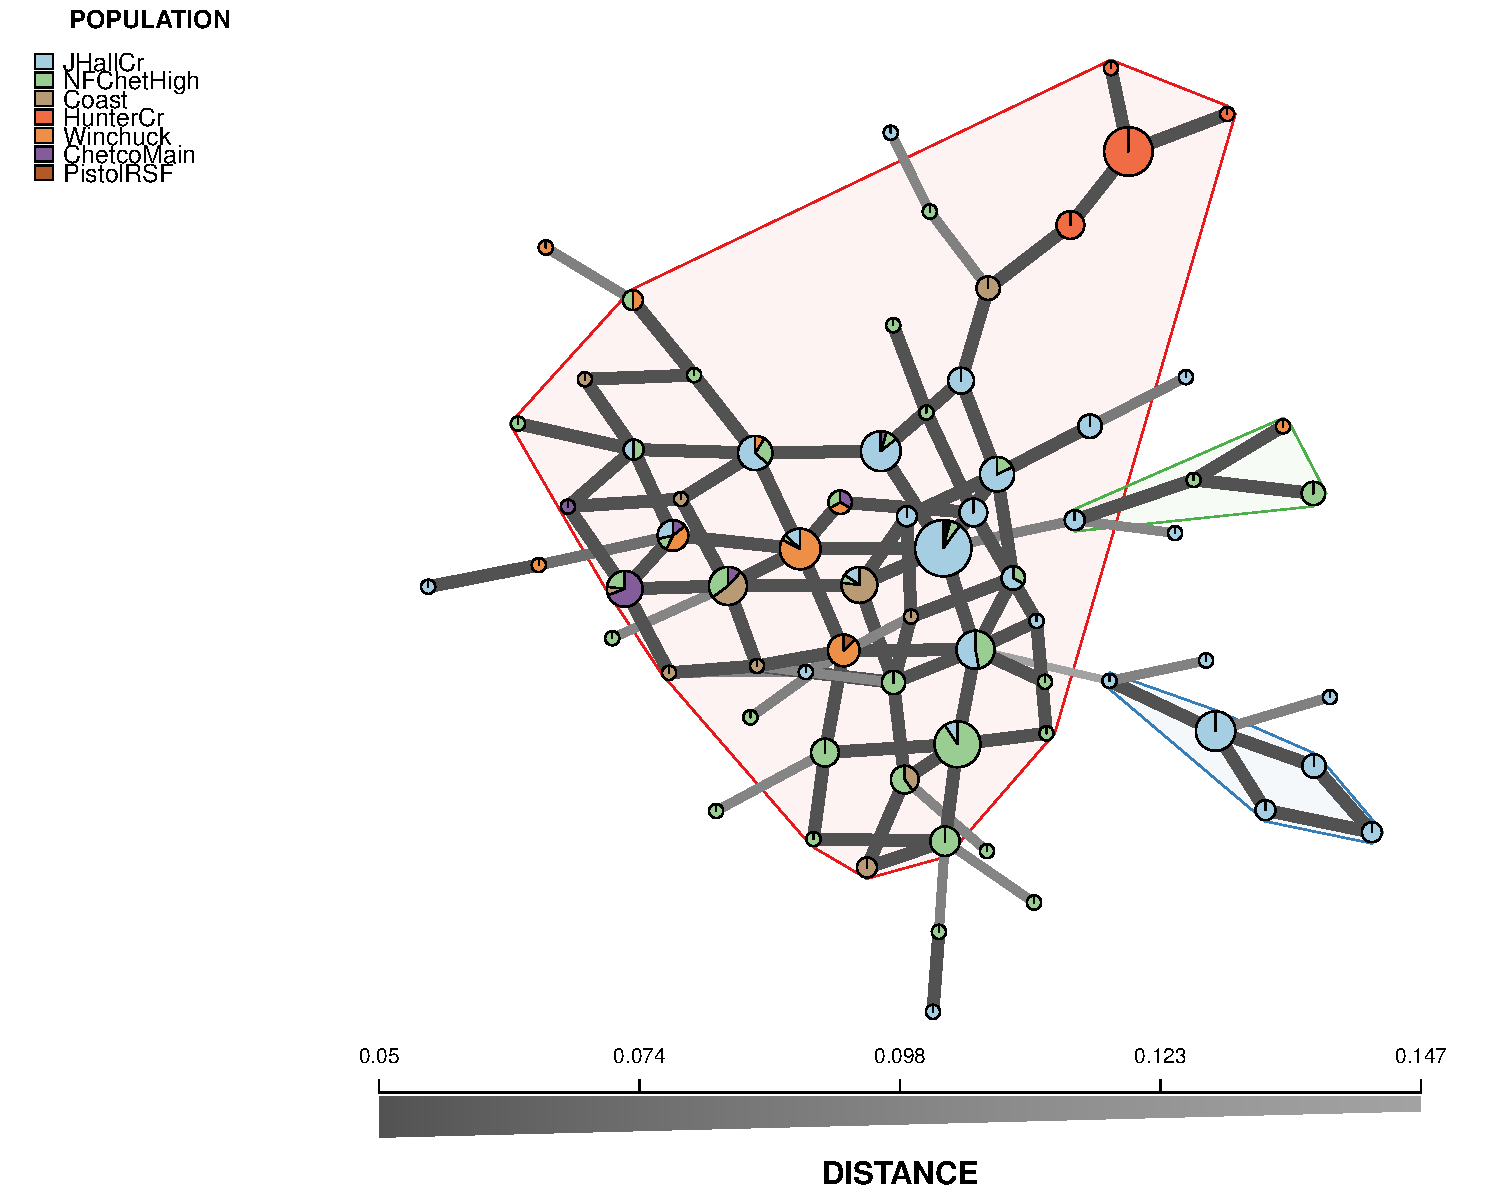
\includegraphics[keepaspectratio, width=0.73\paperwidth]{../msn_forest.png}};
	    \draw<2> [red, ultra thick] (-2.6, -1.05) circle [radius=1];
	\end{tikzpicture}

\end{frame}
%------------------------------------------------------------------------------|
%,,,,,,,,,,,,,,,,,,,,,,,,,,,,,,,,,,,,,,,,,,,,,,,,,,,,,,,,,,,,,,,,,,,,,,,,,,,,,,/


%''''''''''''''''''''''''''''''''''''''''''''''''''''''''''''''''''''''''''''''\
%------------------------------------------------------------------------------|
\begin{frame}[T]

	\begin{center}
		\Huge \bf \sc
		What Happens When
		\vspace{0.3in}
		We Add Nursery Data?
	\end{center}

\end{frame}
%------------------------------------------------------------------------------|
%,,,,,,,,,,,,,,,,,,,,,,,,,,,,,,,,,,,,,,,,,,,,,,,,,,,,,,,,,,,,,,,,,,,,,,,,,,,,,,/



%''''''''''''''''''''''''''''''''''''''''''''''''''''''''''''''''''''''''''''''\
%------------------------------------------------------------------------------|
\begin{frame}[allowpagebreak,T]
	\frametitle{Nei's genetic distance}
	\centering
	\includegraphics[keepaspectratio, height=0.9\paperheight]{../neitree.png}
\end{frame}
%------------------------------------------------------------------------------|
%,,,,,,,,,,,,,,,,,,,,,,,,,,,,,,,,,,,,,,,,,,,,,,,,,,,,,,,,,,,,,,,,,,,,,,,,,,,,,,/


%''''''''''''''''''''''''''''''''''''''''''''''''''''''''''''''''''''''''''''''\
%------------------------------------------------------------------------------|
\begin{frame}[allowpagebreak,T]
	\frametitle{DAPC of forest \& nursery populations}
	\centering
	\includegraphics[keepaspectratio, width=0.85\paperwidth]{../DAPC_nursery.png}
\end{frame}
%------------------------------------------------------------------------------|
%,,,,,,,,,,,,,,,,,,,,,,,,,,,,,,,,,,,,,,,,,,,,,,,,,,,,,,,,,,,,,,,,,,,,,,,,,,,,,,/


%''''''''''''''''''''''''''''''''''''''''''''''''''''''''''''''''''''''''''''''\
%------------------------------------------------------------------------------|
\begin{frame}[allowpagebreak,T]
	\frametitle{MSN of forest \& nursery populations}
	\centering
    \begin{tikzpicture}
	    \node[anchor=north west] at (0,0) {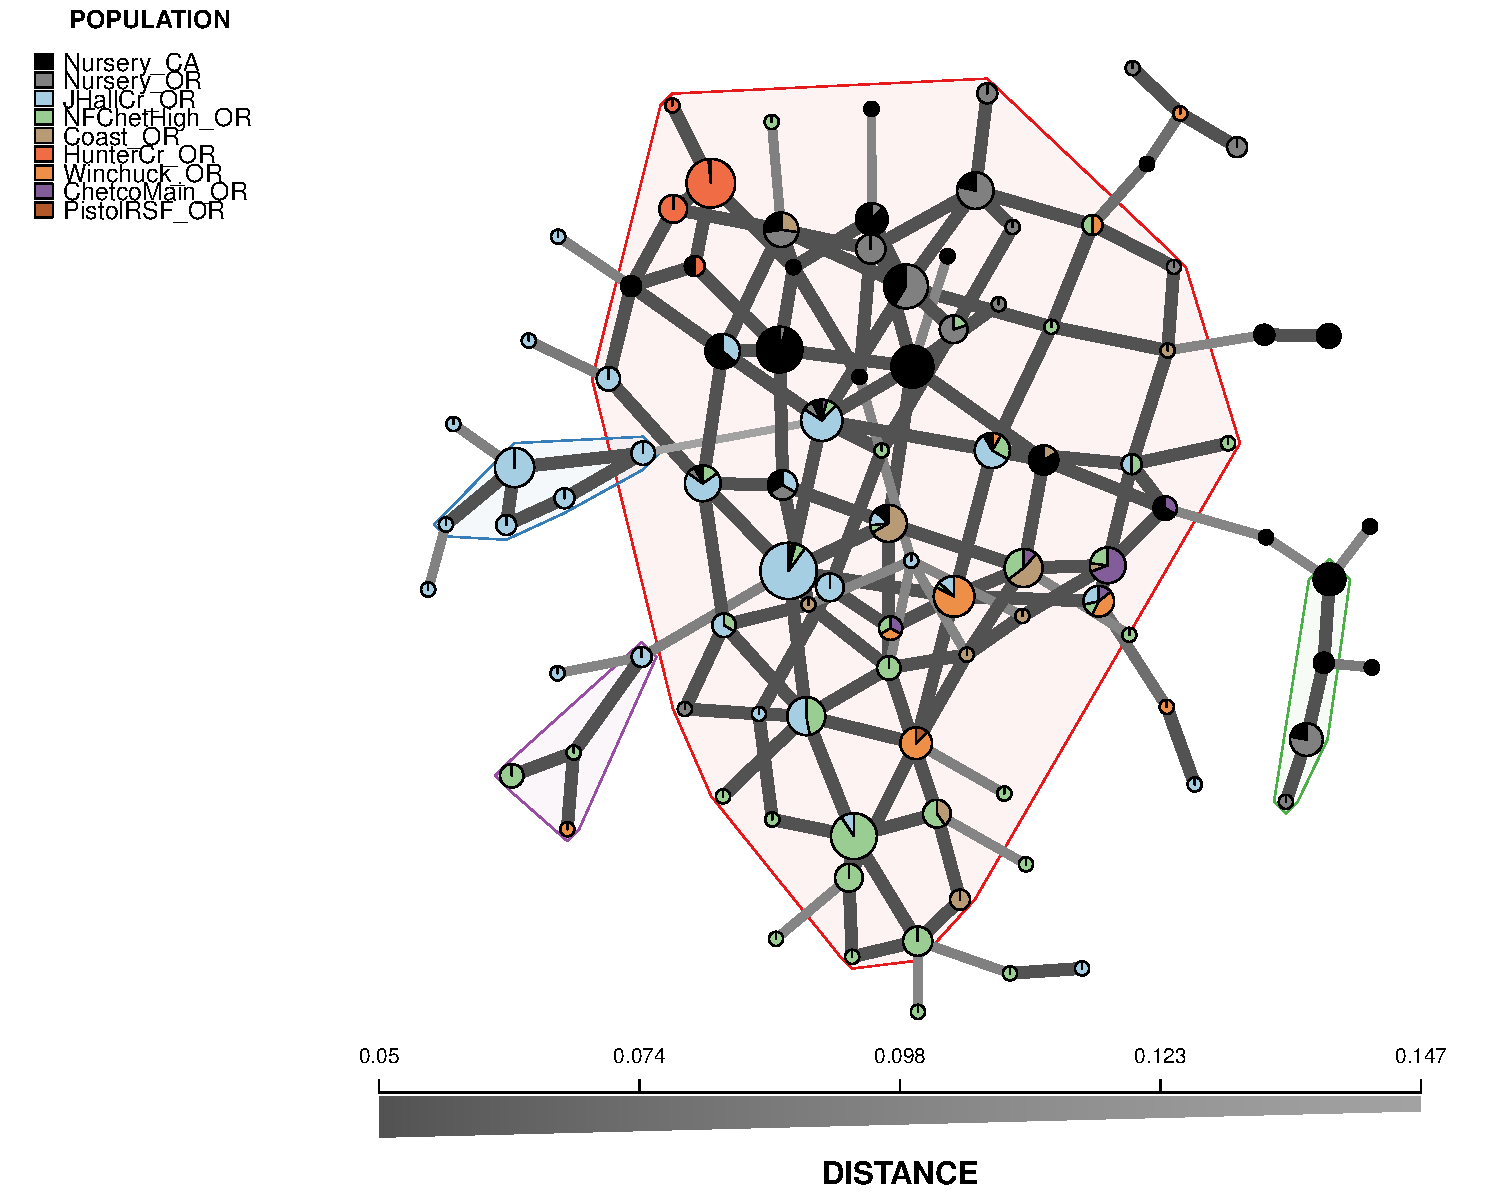
\includegraphics[keepaspectratio, width=0.75\paperwidth]{../msn_both.png}};
	    \draw<2> [red, ultra thick] (4, -1) circle [radius=0.75];
	\end{tikzpicture}

\end{frame}
%------------------------------------------------------------------------------|
%,,,,,,,,,,,,,,,,,,,,,,,,,,,,,,,,,,,,,,,,,,,,,,,,,,,,,,,,,,,,,,,,,,,,,,,,,,,,,,/





%''''''''''''''''''''''''''''''''''''''''''''''''''''''''''''''''''''''''''''''\
%------------------------------------------------------------------------------|
\begin{frame}

	\centering
	\begin{tikzpicture}
		\node (img1) at (0, 0){
			\centering
			\includegraphics[keepaspectratio, height=\paperheight]{figure/PrMS39-1.pdf}
		};
		\node<2>(img2) at (0, -1) {
			\centering
			\includegraphics[width=0.95\paperwidth]{../PrMS39freq.png}
		};
	\end{tikzpicture}

\end{frame}
%------------------------------------------------------------------------------|
%,,,,,,,,,,,,,,,,,,,,,,,,,,,,,,,,,,,,,,,,,,,,,,,,,,,,,,,,,,,,,,,,,,,,,,,,,,,,,,/

\setbeamertemplate{background}
{\includegraphics[width=\paperwidth,height=\paperheight]{../OR_epidemic.png}}
\source{Mike McWilliams, ODF}{white}

\section{Conclusions}
%''''''''''''''''''''''''''''''''''''''''''''''''''''''''''''''''''''''''''''''\
%------------------------------------------------------------------------------|
\begin{frame}
	\begin{center}
		\begin{shaded}
			\Large{\bf \sc Conclusions}
		\end{shaded}
	\end{center}
\end{frame}
%------------------------------------------------------------------------------|
%,,,,,,,,,,,,,,,,,,,,,,,,,,,,,,,,,,,,,,,,,,,,,,,,,,,,,,,,,,,,,,,,,,,,,,,,,,,,,,/

\setbeamertemplate{background}[default]


%''''''''''''''''''''''''''''''''''''''''''''''''''''''''''''''''''''''''''''''\
%------------------------------------------------------------------------------|
\begin{frame}[T]
	\frametitle{What did we find?}
	\Large
	\begin{itemize}
		\item<1-> No new lineages
		\item<2-> Evidence for at least 2 introductions
		\begin{itemize}
			\large
			\item<2-> First in Joe Hall Creek
			\item<2-> Second in Hunter Creek
		\end{itemize}
		\item<3-> These are closely related to nursery genotypes
	\end{itemize}
\end{frame}
%------------------------------------------------------------------------------|
%,,,,,,,,,,,,,,,,,,,,,,,,,,,,,,,,,,,,,,,,,,,,,,,,,,,,,,,,,,,,,,,,,,,,,,,,,,,,,,/

\section*{Acknowledgments}
%''''''''''''''''''''''''''''''''''''''''''''''''''''''''''''''''''''''''''''''\
%------------------------------------------------------------------------------|
\begin{frame}[T]
\frametitle{Acknowledgments}
	\begin{columns}[T]

		\begin{column}{0.5\paperwidth}
			\begin{itemize}
				\item \textbf{Mike McWilliams} -- Aerial Surveys
				\item \textbf{Alan M. Kanaskie} -- GIS work, field surveys, data collection
				\item \textbf{Brookings ground crew} -- data collection, geotagging
				\item \textbf{Hansen Lab} -- Culturing and identification
				\item \textbf{Jen Britt} -- Early genotyping
				\item \textbf{Meredith M. Larsen} -- Genotyping and data harmonization between labs
				\item \textbf{Erica M. Goss} -- Nursery genotypes
			\end{itemize}
		\end{column}

		\begin{column}{0.5\paperwidth}
			\begin{itemize}
				\item USDA-ARS grant 5358-22000-039-00D
				\item USDA-APHIS
				\item USDA-ARS Floriculture Nursery Initiative
				\item ODA/OAN
				\item USDA Forest Service Health Monitoring Program
				\item APS Pacific Division Student Travel Award
			\end{itemize}
		\end{column}

	\end{columns}
\end{frame}
%------------------------------------------------------------------------------|
%,,,,,,,,,,,,,,,,,,,,,,,,,,,,,,,,,,,,,,,,,,,,,,,,,,,,,,,,,,,,,,,,,,,,,,,,,,,,,,/


%%%%%%%%%%%%%%%%%%%%%%%%%%%%%%%%%%%%%%%%%%%%%%%%%%%%%%%%%%%%%%%%%%%%%%%%%%%%%%%%
\appendix
%%%%%%%%%%%%%%%%%%%%%%%%%%%%%%%%%%%%%%%%%%%%%%%%%%%%%%%%%%%%%%%%%%%%%%%%%%%%%%%%


%------------------------------------------------------------------------------|
\begin{frame}
	\begin{center}
	\frametitle{Clonal Lineages}
	\includegraphics[keepaspectratio, width=\textwidth]{../lineages.jpeg}
	\newline
	\mycitep{grunwald2011evolution}
	\end{center}
\end{frame}
%------------------------------------------------------------------------------|



\setbeamertemplate{background}
{\includegraphics[width=\paperwidth,height=\paperheight]{figure/allplots-1.pdf}}

%------------------------------------------------------------------------------|
\begin{frame}[t, allowpagebreak]
	% \centering
	% \includegraphics[keepaspectratio,height=\paperheight]{figure/allplots-1.pdf}
\end{frame}
%------------------------------------------------------------------------------|

\setbeamertemplate{background}[default]

%------------------------------------------------------------------------------|
\begin{frame}[t]
	\frametitle{References}

	\printbibliography
\end{frame}
%------------------------------------------------------------------------------|


\end{document}
